\documentclass[]{article}

\usepackage{amsmath}
\usepackage[]{graphicx}
\usepackage{subfigure}
\usepackage[latin1]{inputenc}
\usepackage{comment}
\usepackage{url}
%\usepackage{biblatex} 
%\usepackage[pdftex]{graphicx}
\usepackage{anysize}

\providecommand{\e}[1]{\ensuremath{\times 10^{#1}}}

\marginsize{3cm}{3cm}{2cm}{2.5cm}%l r t b

\title{Gaze Enhanced Speech Recognition for Hands-Free HCI}
%\title{Controlling a smart phone using gaze gestures}
%\title{Gaze gestures as an innovative HCI method for smartphone like devices}
 
\author{Matheus Portela, David Rozado}

\setlength\parindent{0pt} %no indentation in paragraphs
% Document starts
\begin{document}

\maketitle

\section{Abstract}

In this work, we present an innovative form of correcting misrecognized words during a speech recognition task by using
gaze tracking technology. 


\section{Introduction}
In computer science speech recognition refers to the computational translation of spoken words into text.
Using speech to create or edit documents and e-mail offers the potential to be a faster a more natural way to interact
with computers as well as a hands-free modality with obvious positive implications for handicapped users or
scenarios were computer users have their hands engaged in other tasks (for example surgeons in the operating room).

Although there has been a significant increase in the accuracy performance of speech recognition software, error
rates still make the technology cumbersome to use for everyday interaction and functional speech recognition still
requires a relatively long learning curve on the part of the user to properly master it. Still, misrecognized words
occur often during speech recognition tasks even for advanced users. 

The correction of speech recognition errors or misrecognized words can be carried out manually with a traditional
keyboard and mouse to select and retype the correct word. The usage  of the keyboard and mouse to correct misrecognized
words  during the speech recognition is probably  the most widely used  method for the task. This modality can be
perfectly valid for some scenarios, but this interaction modalities is not trully hands-free anymore.


The usage of voice for correction of misrecognized towards  during the speech recognition maintains the notion of truly
hands-free input to the computer. In practice however, this modality can be very frustrating for the user since
``certain" difficult words are extremely difficult to be properly recognized by speech recognition engines. Hence, this
correction modality is extremely error-prone and frustrating for users. Users with a foreign accent also struggle with
this particular form of interaction. Furthermore repeating several times the same word makes the vocal cords go through
the same pattern of folding and vibrations repeatedly which has been shown to lead to voice strain \cite{}.

 
In this work, we propose the enhancement of speech recognition software with gaze tracking technology to speed up the
correction of misrecognized words and to make speech recognition truly hands-free. A gaze tracking system tracks the
point of regard (PoR) of the user on the screen by monitoring the users pupils while sitting in front of a computer
\cite{Rozado2012a}. In this modality, the user is required to simply gaze at the misrecognized word and then simply
select  the correct alternate  word from an emerging panel for pronounced the word  again the correct option from the
updated on just  by looking at it.


The experimental part of his work compares the three modalities of correcting misrecognized words during  a speech
recognition task:
\begin{itemize}
  \item usage of the traditional keyboard and mouse
  \item usage of voice
  \item usage of gaze
\end{itemize}



%Matheus here you should include the review of the literature


In summary, we present here a multimodal approach to HCI that combines speech recognition with gaze 
interaction for correction of misrecognized words to create a truly hands-free paradigm of inputting text into a
computer. Finally, we explore through a comprehensive user study how this multimodal paradigm compares to the 2
traditional modalities to correct misrecognized words, using voice alone and using the mouse and the keyboard, in terms
of completion task rate, accuracy rate.

\section{Methodology}
Methodology introduction

\subsection{Eye Tracking}
Eyes are used by humans to obtain information about the surroundings and to
communicate information. When something attracts our attention, we position our
gaze on it, thus performing a \textit{fixation}. A fixation usually has a
duration of at least 150 milliseconds (ms). The fast eye movements that
occur between fixations are known as \textit{saccades}, and they are used to
reposition the eye so that the object of interest is projected onto the fovea.
The direction of gaze thus reflects the focus of 
\textit{attention} and also provides an indirect hint for \textit{intention}
\cite{velichkovsky}.


A video-based gaze tracking system seeks to find where a person is looking, i.e.
the Point of Regard (PoR), using images obtained from the eye by one
or more cameras. Most systems employ infrared
illumination that is invisible to the human eye and hence it is not distracting
for the user. Infrared light improves image contrast and produces a reflection
on the cornea, known as corneal reflection or glint. Eye features such as the
corneal reflections and the center of the pupil/iris can be used to estimate the
PoR. Figure \ref{screenGazeTracker} shows a screenshot of an eye being tracked
by the open-source ITU Gaze Tracker \cite{lowcostitugazetracker,Rozado2012}. In this case,
the center of the pupil and two corneal reflections are the features being
tracked.


\begin{figure}[ht]
\begin{center}
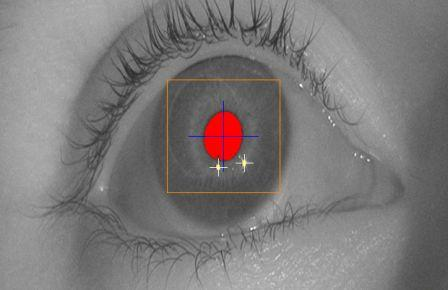
\includegraphics[width=0.5\textwidth, height=30mm]{figures/screenGazeTracker.jpg}
\vspace{-3mm}
\end{center}
\caption{\textbf{The Open Source ITU Gaze Tracker tracking one eye.} The
features tracked in the image are the pupil center and two corneal reflections.}
\label{screenGazeTracker}
\end{figure}


\subsection{Experimental Setup}
The video at \url{http://www.youtube.com/watch?v=xdBoNsMthr8} provides a good overview of the
experimental setup.

\section{Results}
The user study generated the results enumerated next.

The average time  for each correction modality to achieve the target sentence is displayed in Figure \ref{timeFig}.
A Levenes' test for equal variance for the 3 correction modalities failed ($p=2.1$). Hence, the results of the
ANOVA analysis need to be interpreted with caution. The F-test produced a value of $F=17.43$, $p=1.44\e{-06}$.
A Posthoc Bonferroni-Holm test indicated significant differences between the voice-mouse, gaze-mouse and gaze-voice
modalities with $p=4.24\e{-06}$, $p=3.6\e{-05}$ and $p=0.02$, respectively. 
 

\begin{figure}[ht]
\begin{center}
\vspace{-3mm}
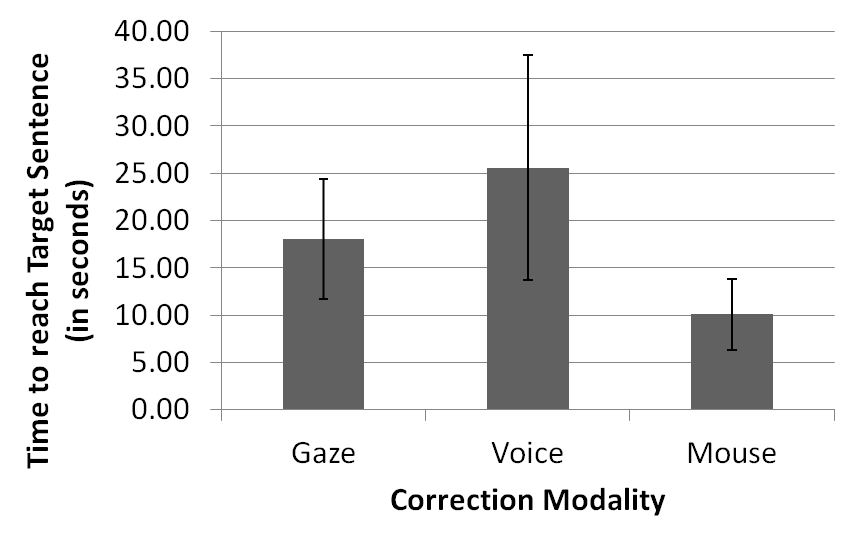
\includegraphics[width=0.95\textwidth,height=50mm]{figures/time.png}
\end{center}
\caption{\textbf{Average Time Required to Achieve Target Sentence.} The figure displays the average time of the
experimental trials required by each correction modality to reach the target sentence.}
\label{timeFig}
\end{figure}


Figure \ref{mouseDisplacement} shows the average displacement of the mouse during each experimental trial for each
correction modality. Again, a Levene's test failed to find equal variance among experimental conditions. The ANOVA
showed significant differences between groups,  $F=25.06$, $p=2.0\e{-08}$. A Posthoc Bonferroni-Holm test found
significant differences between the gaze-mouse and voice-mouse modalities,  $p=1.48\e{-05}$,
$p=1.48\e{-05}$ respectively.


\begin{figure}[ht]
\begin{center}
\vspace{-3mm}
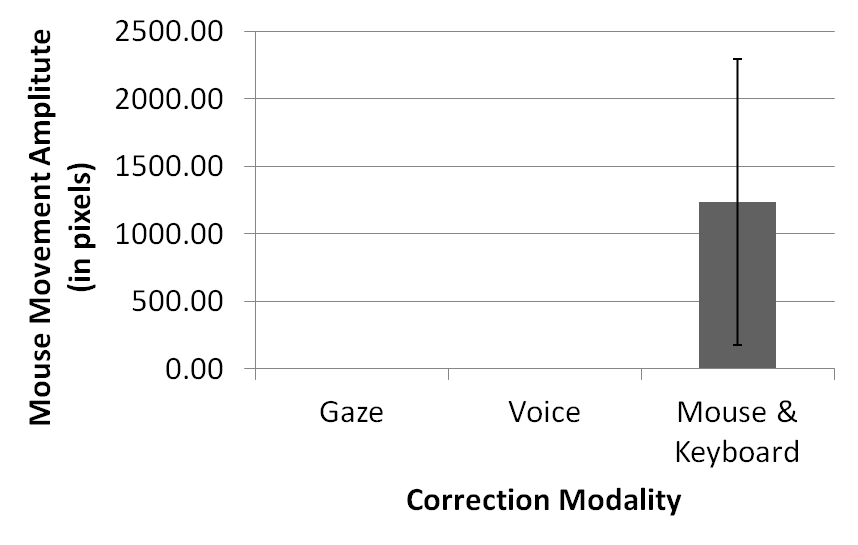
\includegraphics[width=0.95\textwidth,height=50mm]{figures/mouseDisplacement.png}
\end{center}
\caption{\textbf{Average Mouse Movement Amplitude.} The figure displays the average mouse movement amplitude (in pixels)
required by each correction modality to reach the target sentence during the experimental trials.}
\label{mouseDisplacement}
\end{figure}

The average number of keystrokes required from the subjects to achieve the target sentence by each correction modality
during the experimental trials is shown in Figure \ref{keystrokes}. Again a Levene's test failed to assume equal
variance. Nonetheless the ANOVA analysis showed statistically significant differences between the results of the
difference correction modalities, $F=36.79$, $p=8.29\e{-11}$. 

\begin{figure}[ht]
\begin{center}
\vspace{-3mm}
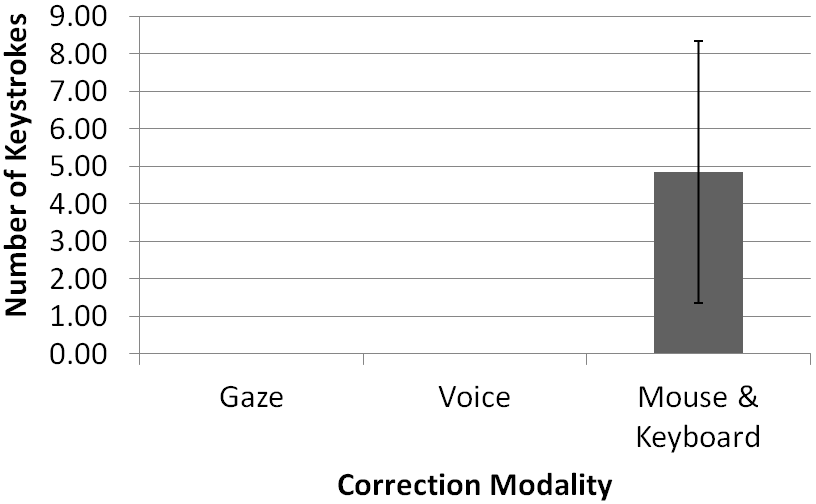
\includegraphics[width=0.95\textwidth,height=50mm]{figures/keystrokes.png}
\end{center}
\caption{\textbf{Number of Keystrokes.} The figure displays the average mouse movement amplitude (in pixels)
required by each correction modality to reach the target sentence during the experimental trials.}
\label{keystrokes}
\end{figure}


Figure \ref{failFig} shows the average number of trials in which the user was unable to reach the target sentence in the
allotted time of 60 seconds using the given correction modality. The Levene's test also failed to determine equal
variance. The ANOVA analysis showed statistically significant differences between the results of the
difference correction modalities, $F=17.92$, $p=1.07\e{-06}$.   A Posthoc Bonferroni-Holm test found
significant differences between the voice-mouse modalities, $p=6.62\e{-06}$, gaze-mouse modalities $p=9.23\e{-05}$
and gaze-voice modalities $p=4.02\e{-03}$.

\begin{figure}[ht]
\begin{center}
\vspace{-3mm}
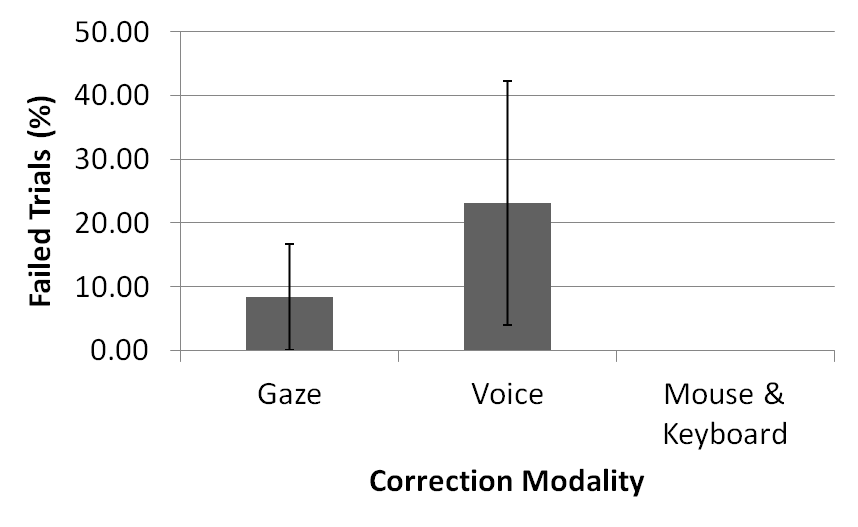
\includegraphics[width=0.95\textwidth,height=50mm]{figures/fail.png}
\end{center}
\caption{\textbf{Number of Failed Trials.} The figure displays the average number of trials in which the user
was unable to reach the given target sentence within the allotted time of 60 seconds.}
\label{failFig}
\end{figure}

The average DL distance between the target sentence and the generated sentence within the 60 seconds time window for
each correction modality is shown in Figure \ref{dldistance}. The ANOVA analysis generated statistically
significant differences between modalities with values $F=11.60$, $p=6.44\e{-05}$. A Posthoc Bonferroni-Holm test found
significant differences between the voice-mouse modalities, $p=5.18\e{-04}$, gaze-voice modalities $p=4.44\e{-03}$
and gaze-mouse modalities $p=1.71\e{-02}$. 

\begin{figure}[ht]
\begin{center}
\vspace{-3mm}
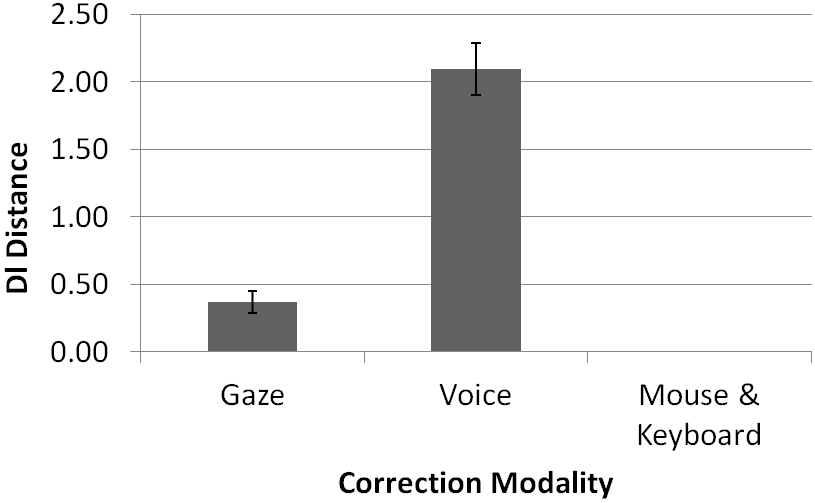
\includegraphics[width=0.95\textwidth,height=50mm]{figures/dldistance.png}
\end{center}
\caption{\textbf{DL Distance.} This figure shows the average DL distance between the target sentence and the generated
sentence.}
\label{dldistance}
\end{figure}


\section{Discussion}
The results of the user study showed that the gaze enhanced correction modality for multimodal speech recognition is not
as fast as using the mouse and the keyboard for correcting misrecognized words. Yet, the gaze modality is
significantly faster that using voice alone for correction and it is trully hand-free as opposed to the Mouse\&Keyboard
modality that required the usage of the hands for correction misrecognized words.

The amount of mouse movement displacement to achieve the target sentence was obviously non-existant for the gaze and
voice correction modalities due to their true hands-free nature. The same can be say of the amount of keystrokes presses
required for correction.

In terms of the number of failures registered during the experimental trials to achieve the target sentence, the gaze
modality was significantly better at reaching the target sentence that the voice modality but worse than the mouse \&
keyboard modality. This was also evident in the DL distance between the target sentence and the achieved sentence during
the experimental trials.

In conclusion, the gaze modality for correction of recognized words is not as efficient in terms of accuracy and time to
completion as the traditional mouse \& keyboard modality but it possesses the advantage of being truly hand-free with
obvious  implications for handicapped computer users, users suffering from RSI syndrome and for scenarios where the
usage of the hands is not possible (surgery room for instance). Moreover, the gaze modality significantly outperforms
the other hand-free modality to correct misrecognized words, using voice, in all the variable being monitor in the user
study. Furthermore, the gaze based correction modality also prevents the appearance of voice strain for the correction
of misrecognized words since it prevents the  repetition of utterances of a certain word.

The evidence from the results presented here suggest the advantages of this multimodal approach to HCI that complements
speech recognition with gaze tracking and gaze interaction to create a truly hands-free multimodal interface that is
faster and more accurate than using voice alone to correct misrecognized words.


\bibliographystyle{plain}
\bibliography{library}

\end{document}
